%% Last modified: Time-stamp: <2011-06-23 22:21:56 (srdbadmin)>
%% a single pdf with all the figures for the Fish and Fisheries June 24 2011 resubmission
\documentclass[letterpaper,12pt]{article}
\usepackage{pdflscape}
\usepackage{graphicx}

\pagestyle{empty}

\begin{document}

\noindent Figure 1. Temporal coverage of a) catch/landings, b) spawning stock biomass and c) recruitment. The temporal coverage for individual assessments is represented by thin alternating black and grey horizontal lines in the main panels. Thick horizontal lines at the base of each main panel represent the time periods that are present in 90\% (black) and 50\% (grey) of all series for that data type. Subfigure histograms contain the frequency of occurrence of the various timespans without reference to time period. Solid and long-dash vertical lines within the subfigures represent the median, 2.5\% and 97.5\% quantiles, respectively.
\\

\noindent Figure 2. Map of Large Marine Ecosystems (LMEs) and high seas areas (ovals) showing the number of stock assessments present in the database per area. 
\\

\noindent Figure 3. Comparison of the taxonomic diversity of marine species as provided by a)
FishBase, b) the coverage of catch data as provided by the Sea Around Us
Database, and c) the new RAM Legacy database (bottom panel). The circle
located near the middle of the circular dendrogram represents kingdom Animalia and
each subsequent branching represents a different taxonomic group (Kingdom to Phylum
to Class to Order to Family to Genus to Species). The width of each line is proportional
to the square root of the number of species in a branch. To facilitate the identification
of the taxonomic groups that are not presented in the catch and assessment data, the
FishBase branching pattern of the spoked dendrogram is maintained to generate the
other two dendrograms. This figure only compares fish and elasmobranch species present in FishBase. Additional species of molluscs and arthropods are present in both the Sea Around Us and RAM Legacy databases but are not presented here.
\\

\noindent Figure 4.  Current exploitation rate versus current biomass for individual stocks from a) all management units combined (updated from Worm et al. 2009) and for b-i) individual management units b) U.S., c) New Zealand, d)Australia, e) Europe, f) Canada, g) Atlantic (multinational stocks managed by ICCAT and NATO), h) Pacific (including multinational stocks managed by IATTC, WCPFC and SPRFMO), and i) others. In each panel, exploitation rate is scaled relative to the exploitation rate expected to result in maximum sustainable yield ($U_{msy}$); biomass is scaled relative to $B_{msy}$. Shading indicates the probability of occurrence as revealed by a kernel density smoothing function. Solid circles indicate and estimates that were obtained directly from assessments; open circles indicate estimates from surplus production models. 
\\

\noindent Figure 5.  Current exploitation rate versus current biomass for individual stocks from the major orders of marine fishes a) Gadiformes, b) Decapoda, c) Scorpaeniformes, d) Perciformes, e) Pleuronectiformes and f) Clupeiformes, in the RAM Legacy database. Plot details as in Figure 4.
\\

\noindent Figure 6.  Current exploitation rate versus current biomass for individual stocks from a) low (>=2.0 - <3.0), b) medium (>=3.0 - <4.0) and c) high (>=4.0) trophic levels. Plot details as in Figure 4.


\begin{landscape}
\begin{figure}
\begin{center}
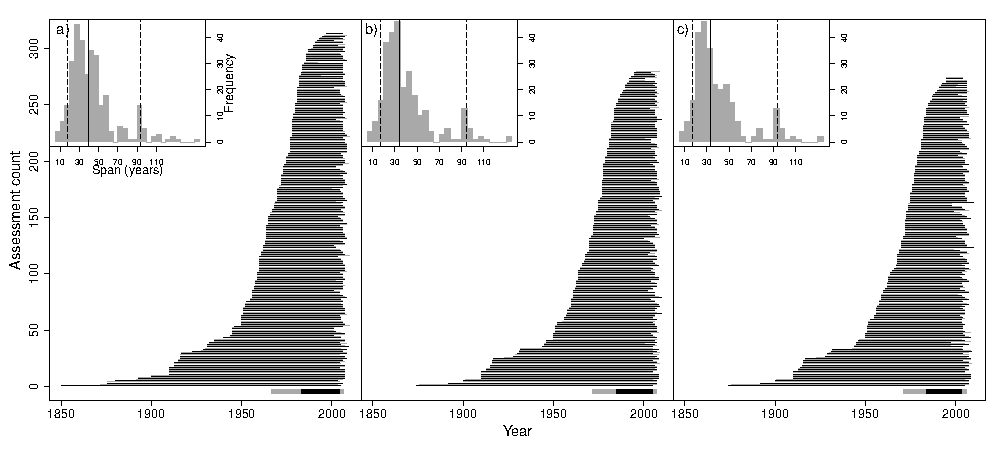
\includegraphics[width=8in]{/home/srdbadmin/srdb/projects/fishandfisheries/R/first-review/orca-plot.pdf}
\end{center}
\caption{ }\label{fig:orca}
\end{figure}
\end{landscape}

\begin{landscape}
\begin{figure}
\begin{center}
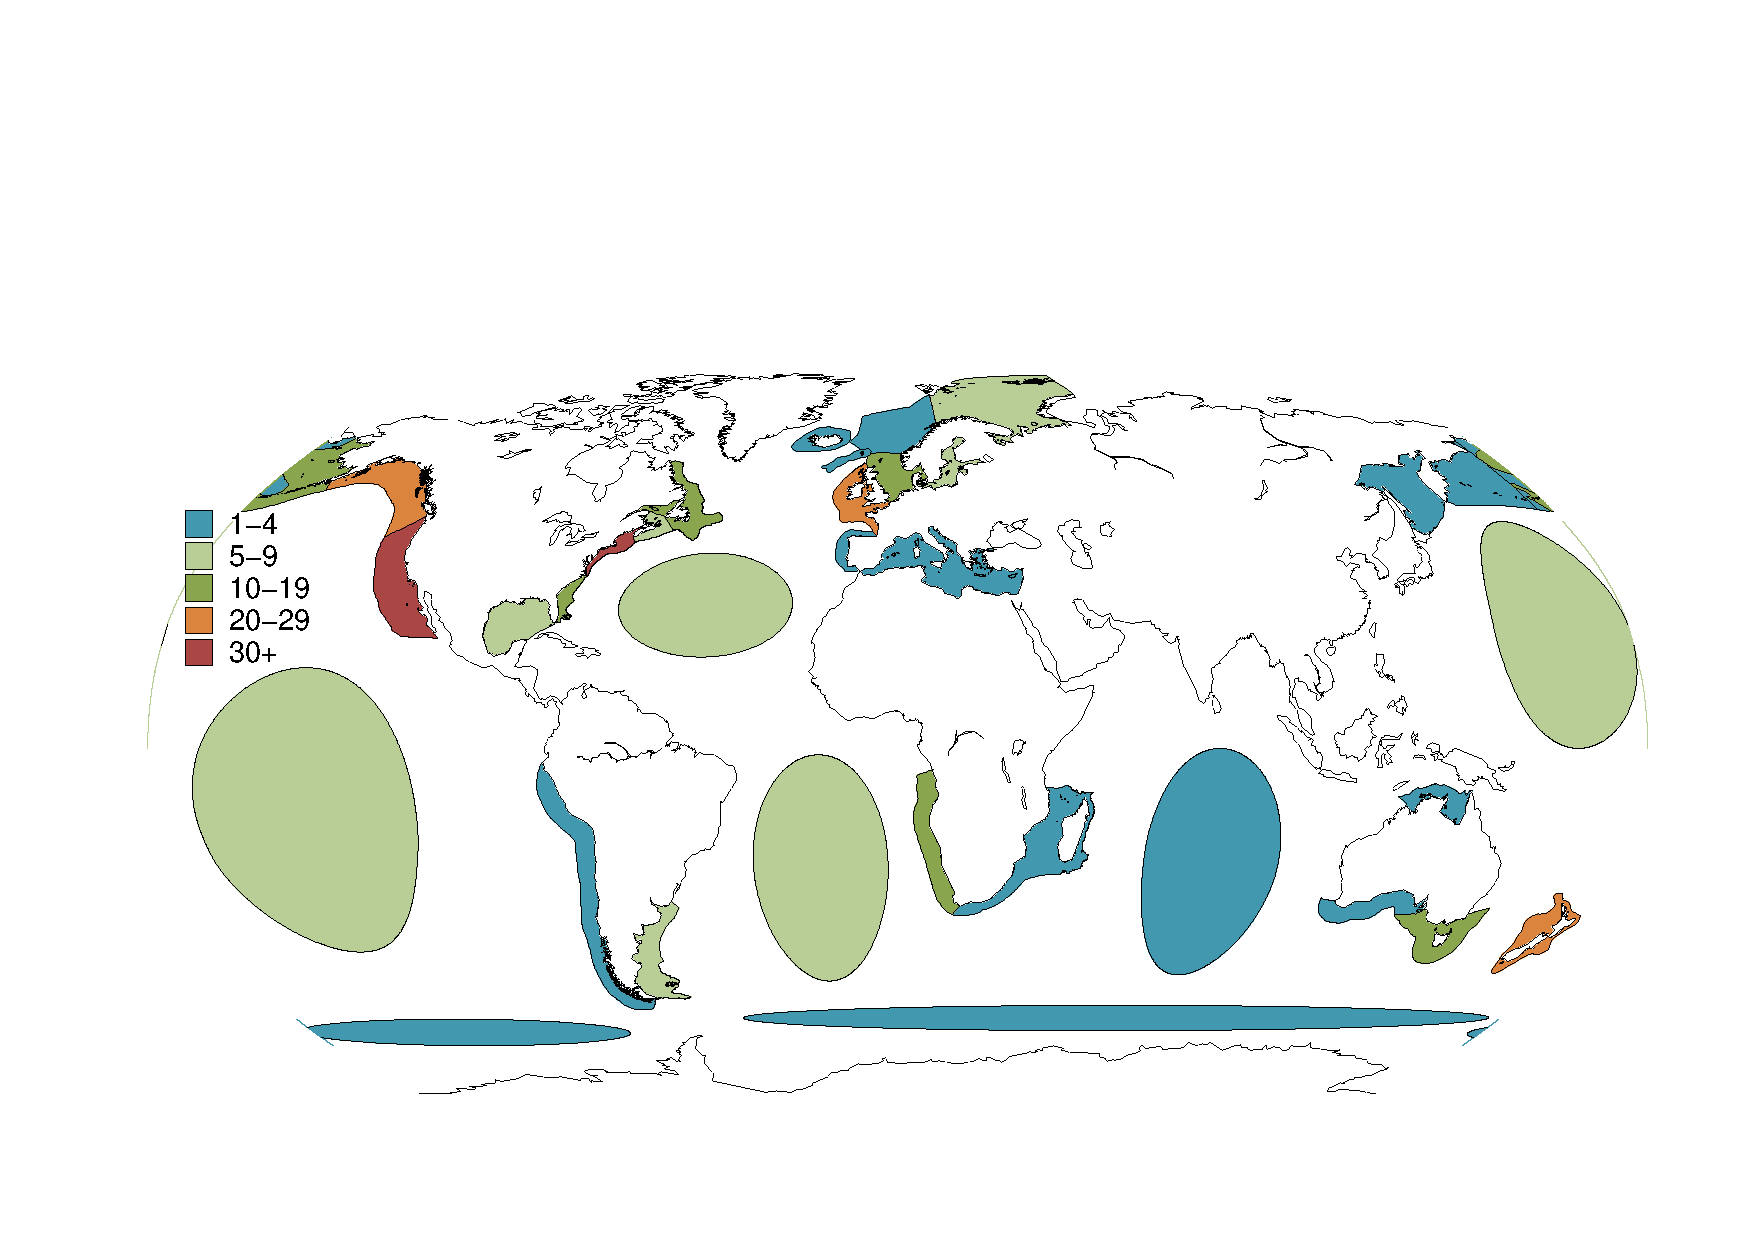
\includegraphics[width=8in]{/home/srdbadmin/srdb/projects/fishandfisheries/GMT/stocks-byLME.pdf}
\end{center}
\caption{ }\label{fig:lmes}
\end{figure}
\end{landscape}


\begin{figure}
\begin{center}
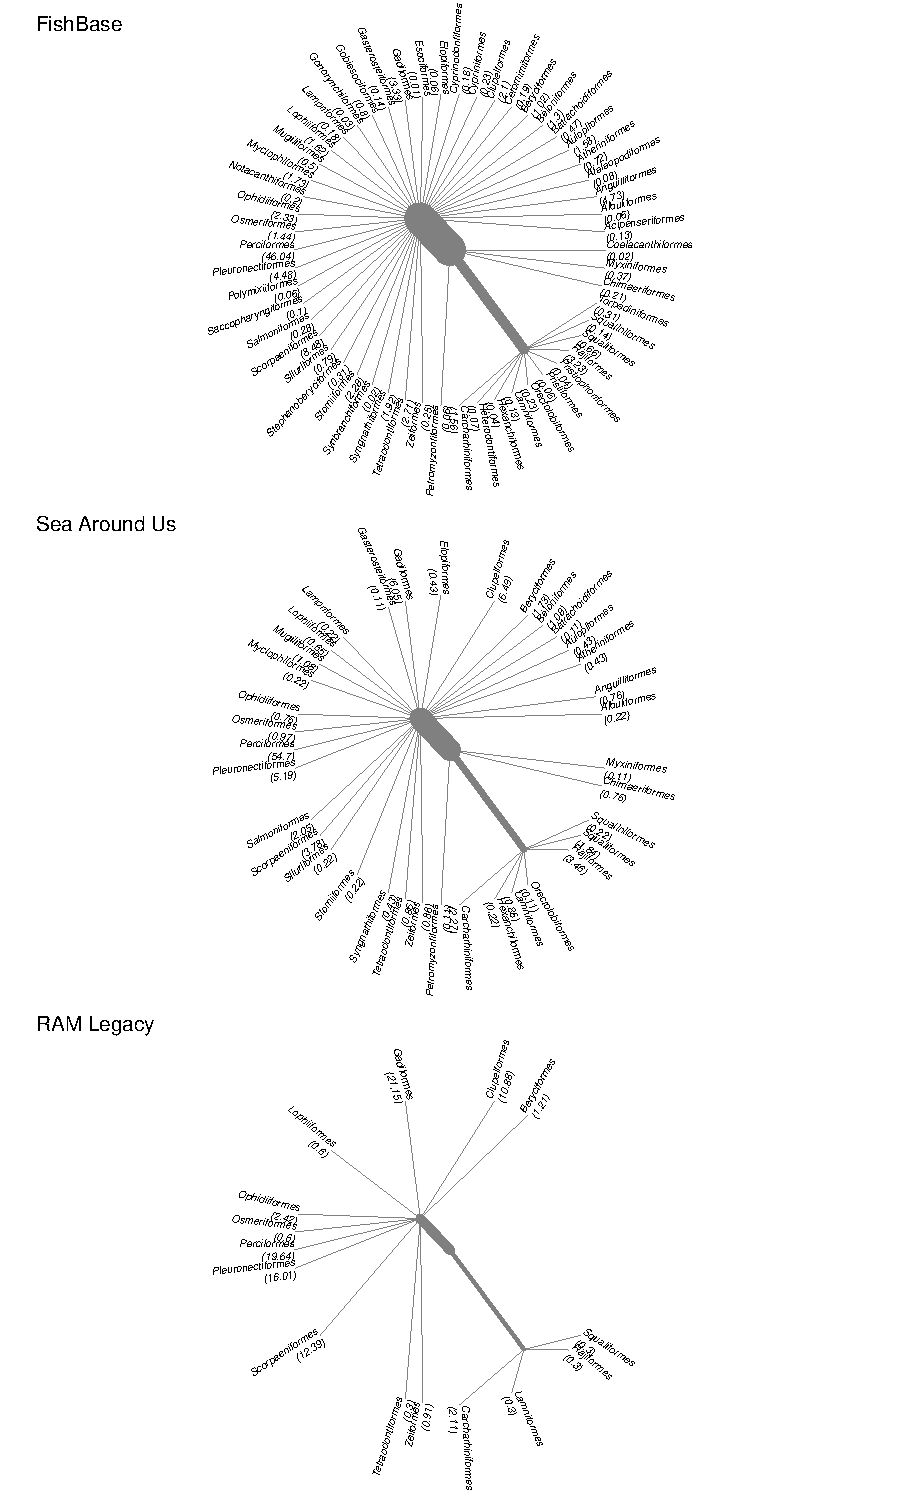
\includegraphics[height=8.5in]{/home/srdbadmin/srdb/projects/fishandfisheries/R/first-review/three-panel-phylo.pdf} % fishbase_saup_two_panel_phylo.pdf}
\end{center}
\caption{ }\label{fig:taxo:threepanel}
\end{figure}


\begin{landscape}
\begin{figure}
\begin{center}
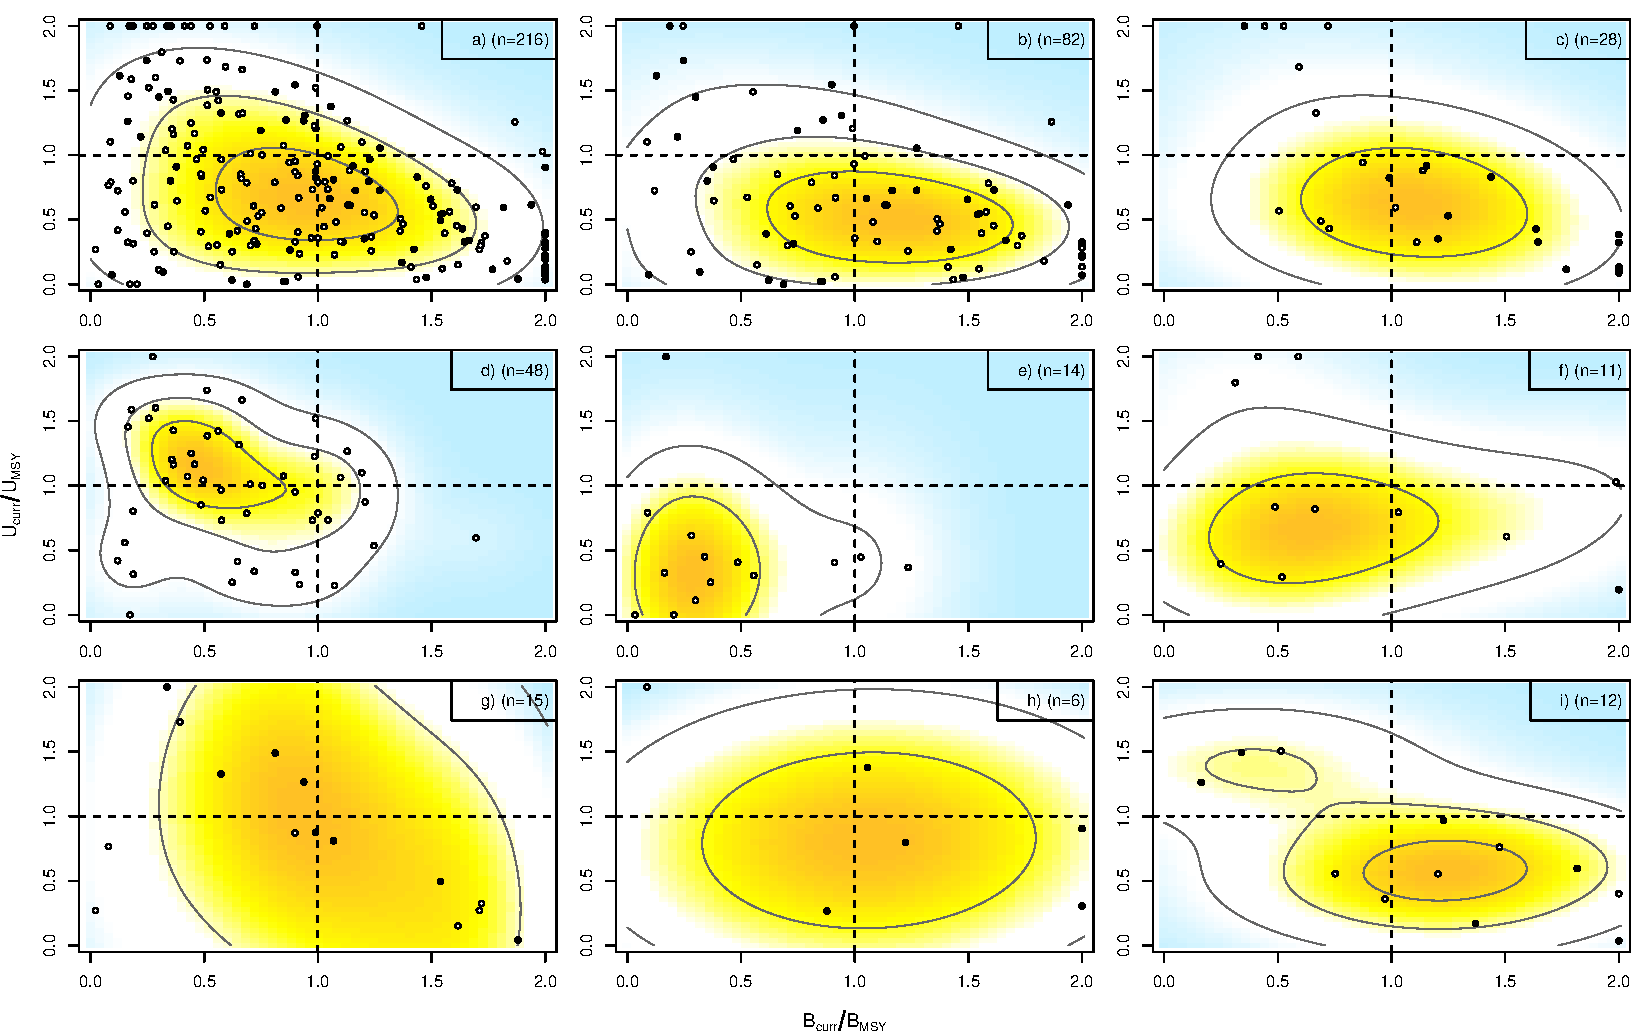
\includegraphics[width=9in]{/home/srdbadmin/srdb/projects/fishandfisheries/R/first-review/friedegg-9plots-fandf.pdf}
\end{center}
\caption{ }\label{fig:friedegg}
\end{figure}
\end{landscape}

%For the top 6 taxonomic orders (Figure~\ref{fig:taxo}).
\begin{figure}
\begin{center}
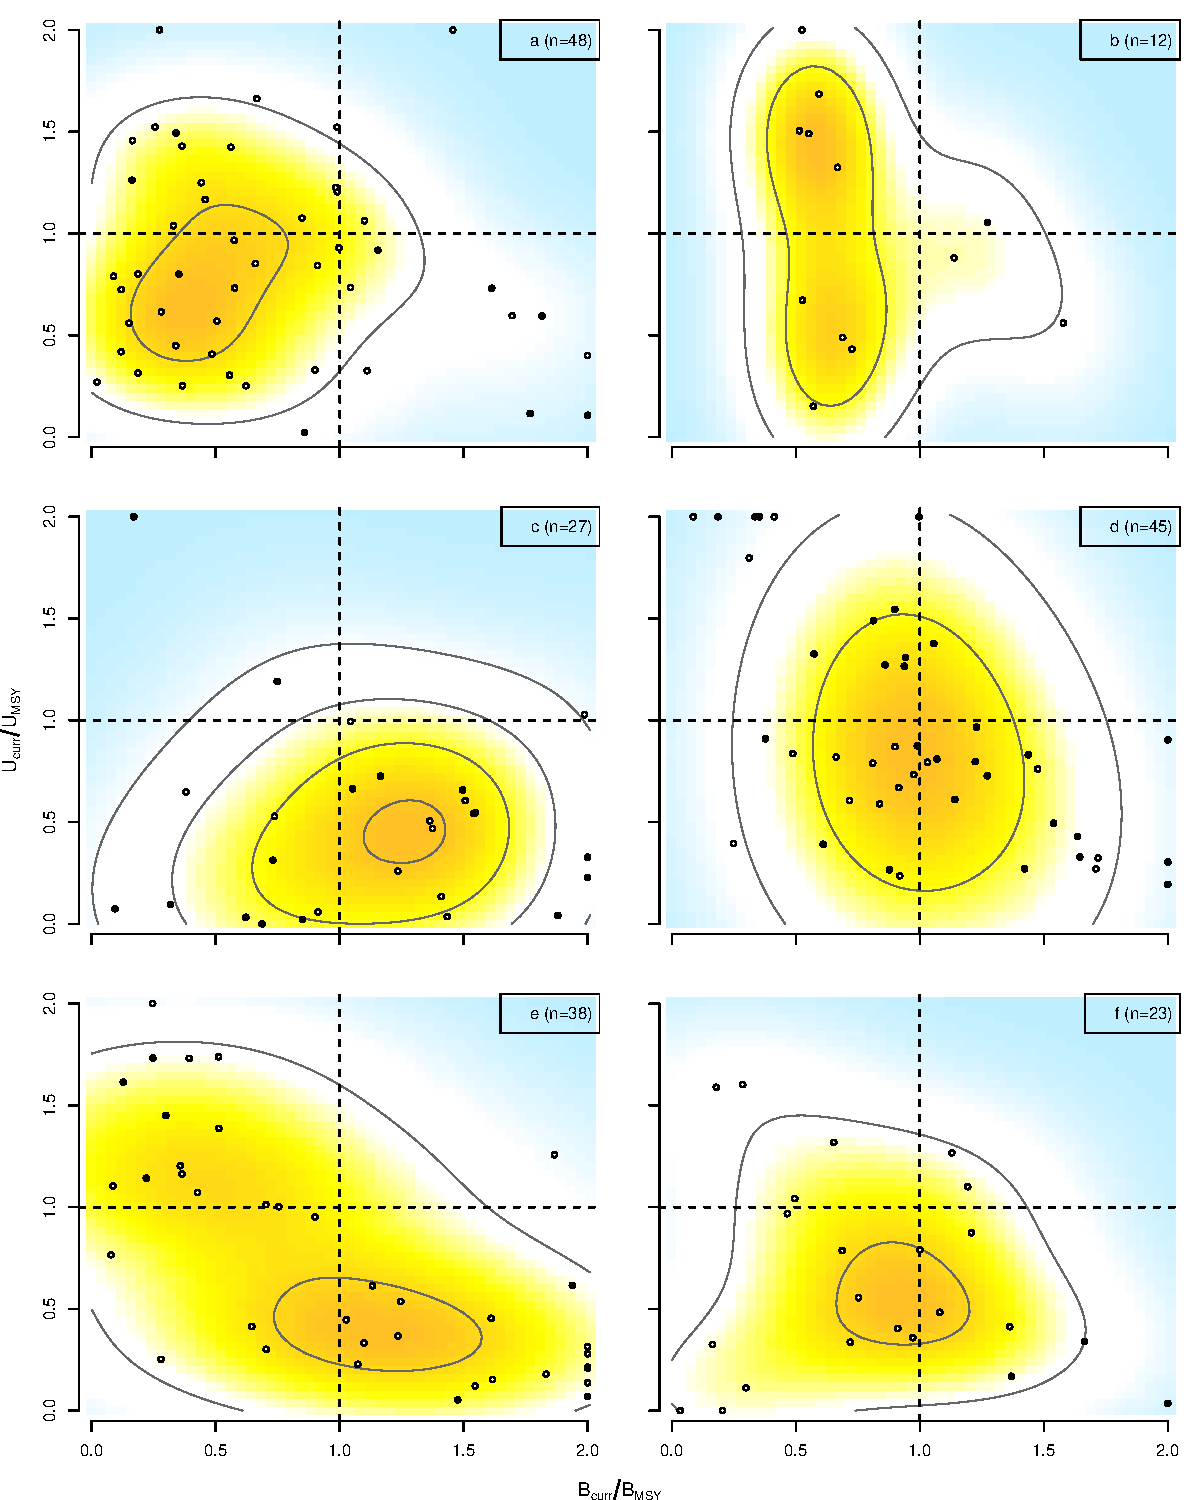
\includegraphics[width=15cm]{/home/srdbadmin/srdb/projects/fishandfisheries/R/first-review/friedegg-taxo.pdf}
\end{center}
\caption{ }
\label{fig:taxo}
\end{figure}

%By trophic level (Figure~\ref{fig:mtl}).

\begin{landscape}
\begin{figure}
\begin{center}
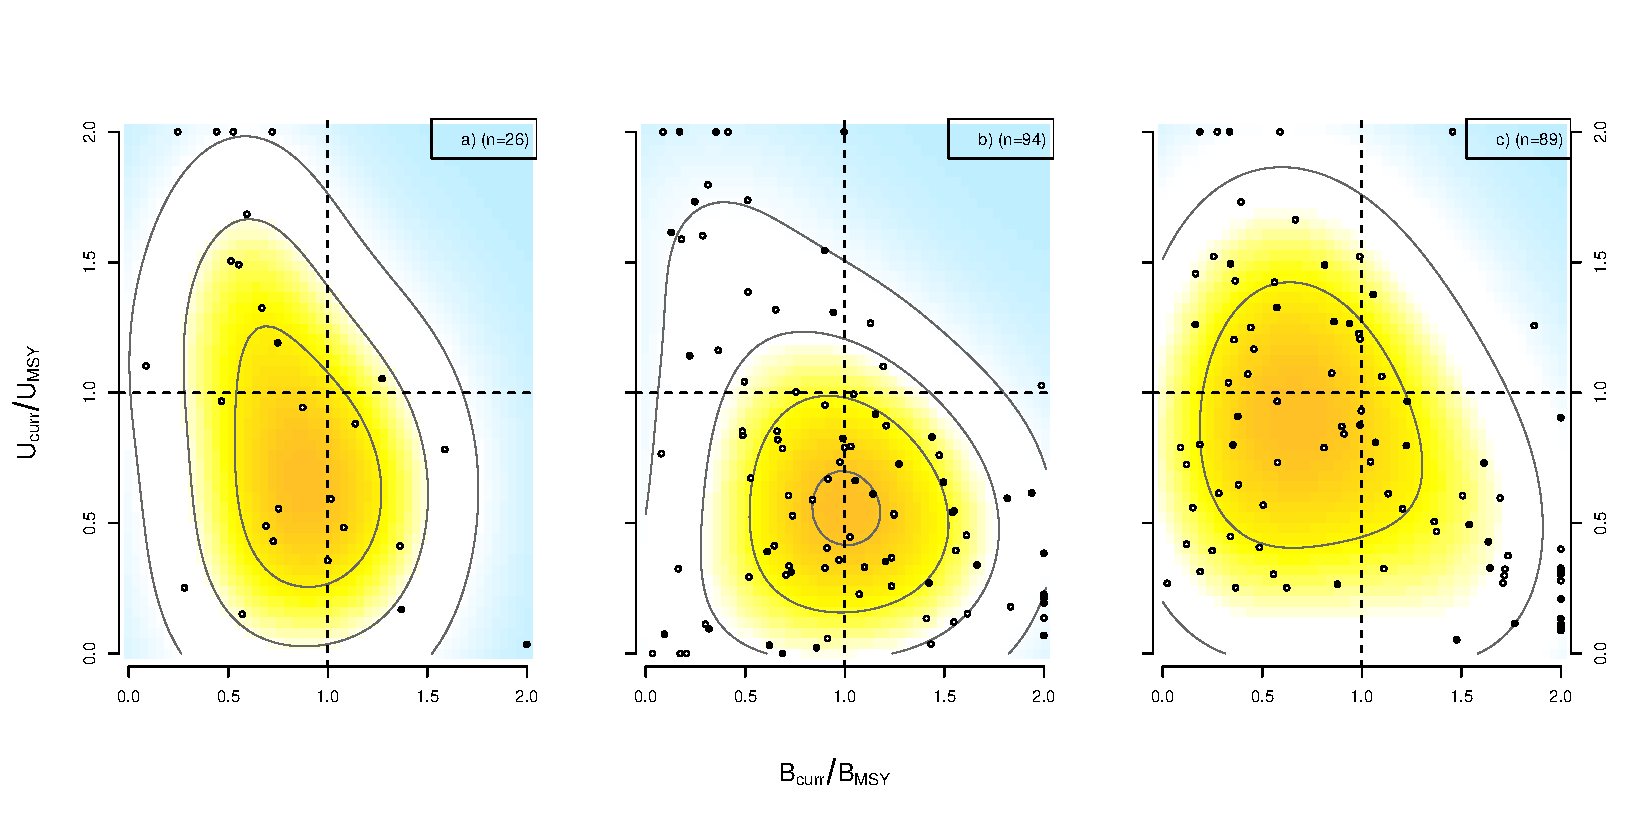
\includegraphics[width=20cm]{/home/srdbadmin/srdb/projects/fishandfisheries/R/first-review/friedegg-MTLs.pdf}
\end{center}
\caption{ }
\label{fig:mtl}
\end{figure}
\end{landscape}

\end{document}
